\documentclass[tikz]{standalone}
\usepackage{pgfplots}
\pgfplotsset{compat=1.15}
\usepackage{mathrsfs}
\usetikzlibrary{arrows,calc}
\usepackage{tkz-euclide}
\pagestyle{empty}

\definecolor{AngleClr}{rgb}{0,0.39215686274509803,0}
\definecolor{ShapeClr}{rgb}{0.6,0.2,0}

\begin{document}

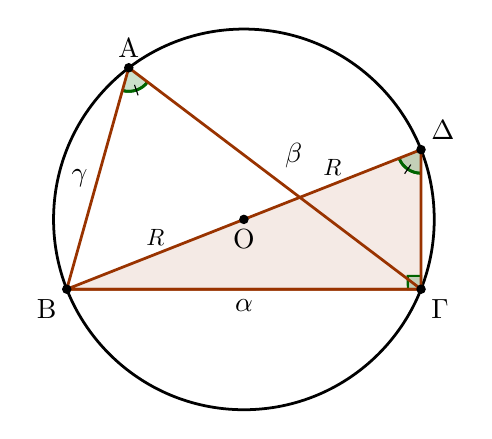
\begin{tikzpicture}[scale=.75]
\tkzSetUpLine[line width=1pt,color=black]
\tkzSetUpPoint[fill=black]

\tkzDefPoints{0/0/A,6/0/B,1.05/3.75/C}

\tkzDefCircle[circum](A,B,C) \tkzGetPoint{O}
\tkzDefPointBy[symmetry=center O](A) \tkzGetPoint{D}
\tkzDrawCircle[line width=1.0pt, color=black](O,A)

\tkzFillPolygon[fill=white](A,B,C)

\tkzFillPolygon[fill=ShapeClr,fill opacity=0.1](A,B,D)

\tkzFillAngles[fill=AngleClr,size=.4,fill opacity=0.2](A,C,B A,D,B)
\tkzMarkAngles[line width=1pt,size=.4,color=AngleClr](A,C,B A,D,B)
\tkzMarkAngles[line width=1pt,size=.4,color=AngleClr,mark=|,mksize=2](A,C,B A,D,B)

\tkzMarkRightAngle[line width=0.75pt, size=.225,color=AngleClr,fill=AngleClr,fill opacity=0.2](A,B,D)



\tkzDrawPolygon[color=ShapeClr](A,B,C)
\tkzDrawPolygon[color=ShapeClr](A,B,D)

\tkzDrawPoints[size=3](A,B,C,D,O)
\tkzLabelPoint[above](C){$\rm A$}
\tkzLabelPoint[below left](A){$\rm B$}
\tkzLabelPoint[below right](B){$\rm \Gamma$}
\tkzLabelPoint[above right](D){$\rm \Delta$}
\tkzLabelPoint[below](O){$\rm O$}

\tkzLabelSegment[left](A,C){$\gamma$}
\tkzLabelSegment(A,B){$\alpha$}
\tkzLabelSegment[above right](B,C){$\beta$}

\tkzLabelSegment[above,scale=0.85](O,A){$R$}
\tkzLabelSegment[above,scale=0.85](O,D){$R$}

\end{tikzpicture}
\end{document}
